\chapter{Solu\c{c}\~ao das Equa\c{c}\~oes \ref{eq.matricial_1}-\ref{eq.matricial_4} na Aus\^encia de Fonte}\label{sec.ausencia_fonte}

Vamos determinar inicialmente a solu\c{c}\~ao das equa\c{c}\~oes \ref{eq.matricial_1}-\ref{eq.matricial_4} considerando o meio homog\^eneo e livre de fonte de onda sismica. Apos a diagonalizacao dessas equacoes, podemos aplicar um m\'etodo utilizado por alguns autores como \cite{Ursin-1983}, \cite{Azeredo_2013}, \cite{White_Zhou_2006}, \cite{miranda_2016} entre outros, para determinar as solu\c{c}\~oes na aus\^encia de fonte. Esse mesmo metodo pode ser utilizado para determinar as solucoes na presenca de fonte como veremos no capitulo \ref{sec.presenca_fonte}. Aus\^encia de fonte significa que temos $\mathbf{S}^{(m)}=0$ para $m=1,2,3,4\,$ na equa\c{c}\~ao \ref{eq.matricial}. A matriz $\mathbf{M}^{(m)}$ \'e constante onde as submatrizes na diagonal principal s\~ao nulas e as submatrizes na diagonal secund\'aria s\~ao sim\'etricas. 



\section{Ondas Ascendentes e Ondas Descendentes}

Vamos redefinir o vetor de ondas como
\begin{equation}\label{eq.Phi}
\mathbf{\Phi}=L\,\mathbf{\Psi}.
\end{equation}
Substituindo a equa\c{c}\~ao \ref{eq.Phi} na equa\c{c}\~ao \ref{eq.matricial}, temos
\begin{equation}\label{eq.matricial_sem_fonte}
\frac{\partial\,\mathbf{\Psi}}{\partial\,z} =-\,i\,\omega\,L^{-1}M\,L\,\mathbf{\Psi},
\end{equation}
onde o sobrescrito $m$ est\'a sendo omitido por quest\~ao de simplicidade.
De acordo com a subse\c{c}\~ao \ref{sec.diagonalizacao_ursin}, temos que as matrizes $M$ e $\tilde{\Lambda}$ s\~ao semelhantes, assim
\begin{equation*}
\tilde{\Lambda}=L^{-1}M\,L.
\end{equation*}
Substituindo $\tilde{\Lambda}$ na equa\c{c}\~ao \ref{eq.matricial_sem_fonte}, temos
\begin{equation}\label{eq.matricial_sem_fonte_2}
\frac{\partial\,\mathbf{\Psi}}{\partial\,z} =-\,i\,\omega\,\tilde{\Lambda}\,\mathbf{\Psi}.
\end{equation}
Ainda de acordo com a subse\c{c}\~ao \ref{sec.diagonalizacao_ursin}, podemos escrever
\begin{equation}
\tilde{\Lambda}=
\begin{pmatrix}
\Lambda&0\\
0&-\Lambda
\end{pmatrix},
\end{equation}
onde $\Lambda$ \'e uma submatriz diagonal contendo os autovalores $q_i$.
Definindo
\begin{equation}\label{eq.definicao_psi}
\mathbf{\Psi}=
\begin{pmatrix}
\mathbf{U}\\
\mathbf{D}
\end{pmatrix}
\end{equation}
e usando o fato de que $\tilde{\Lambda}$ \'e uma matriz diagonal, podemos resolver a equa\c{c}\~ao diferencial \ref{eq.matricial_sem_fonte_2} e expressar a solu\c{c}\~ao na forma
\begin{align}\nonumber
\mathbf{\Psi}(z)&=e^{-i\,\omega\,\tilde{\Lambda}(z-z_0)}\mathbf{\Psi}(z_0)\\\label{eq.solucao_psi}
&=\begin{pmatrix}
e^{-i\,\omega\,\Lambda(z-z_0)}\,\mathbf{U}(z_0)\\
e^{i\,\omega\,\Lambda(z-z_0)}\,\,\,\mathbf{D}(z_0)
\end{pmatrix}.
\end{align}
Desta maneira, $\mathbf{U}$ representa ondas ascendentes e $\mathbf{D}$ representa ondas descendentes, $z_0$ \'e um ponto fixo na mesma regi\~ao livre de fonte de $z$ e $e^{\pm i\,\omega\,\Lambda(z-z_0)}$ \'e uma matriz diagonal onde o $i$-ésimo elemento da diagonal principal \'e dado por $e^{\pm i\,\omega\,q_i(z-z_0)}$. 

\section{Matriz de Salto para Camadas Estratificadas}

A profundidade onde encontra-se uma interface entre duas camadas estratificadas ser\'a denotada por $\overline{z}$, onde as quantidades avaliadas exatamente abaixo da interface ser\'a denotada por $\overline{z}^+$ e as quantidades avaliadas exatamente acima da interface ser\'a denotada por $\overline{z}^-$.
De acordo com TAL, temos a continuidade de $\mathbf{\Phi}$ atrav\'es das fronteiras entre as camadas, assim \'e v\'alida a rela\c{c}\~ao $\mathbf{\Phi}^+=\mathbf{\Phi}^-$. Substituindo a equa\c{c}\~ao \ref{eq.Phi}, temos 
\begin{align}\nonumber
L^+\mathbf{\Psi}^+&=L^-\mathbf{\Psi}^-\\\nonumber
\mathbf{\Psi}^+&=(L^+)^{-1}L^-\mathbf{\Psi}^-\\\label{eq.psi_matriz_salto}
\mathbf{\Psi}^+&=J\,\mathbf{\Psi}^-,
\end{align}
onde $J=(L^+)^{-1}L^-$ \'e denominada \textit{matriz de salto}. Pela subse\c{c}\~ao \ref{sec.diagonalizacao_ursin} podemos verificar que
\begin{equation}\label{eq.matriz_L}
L=\frac{1}{\sqrt{2}}
\begin{pmatrix}
L_1&L_1\\
L_2&-L_2
\end{pmatrix},
\end{equation}
e podemos expressar a matriz de salto como
\begin{equation}
J=
\begin{pmatrix}
J_A&J_B\\
J_B&J_A
\end{pmatrix},
\end{equation}
onde $J_A$ e $J_B$ s\~ao dadas por
\begin{align}\label{eq.j_a}
J_A&=\frac{1}{2}\left[(L_2^+)^\top L_1^-+(L_1^+)^\top L_2^-\right]\\\label{eq.j_b}
J_B&=\frac{1}{2}\left[(L_2^+)^\top L_1^--(L_1^+)^\top L_2^-\right].
\end{align}
Com uma simples multiplica\c{c}\~ao de matrizes temos que
\begin{align}\nonumber
J^{-1}&=(L^-)^{-1}L^+\\\label{eq.inversa_matriz_salto}
&=
\begin{pmatrix}
J_A^\top&-J_B^\top\\
-J_B^\top&J_A^\top
\end{pmatrix}.
\end{align}

\section{Matriz de Reflex\~ao e Matriz de Transmiss\~ao}

Considere um meio estratificado, homog\^eneo no interior de cada camada, com $N$ interfaces nas profundidades $0<z_1<z_2<...<z_N<\infty$ e sem exist\^encia de fonte nessas camadas. 

\subsection{Reflex\~ao e Transmiss\~ao na \'Ultima Interface}
Pela figura \ref{fig.ondas_em_zn}, considerando que n\~ao h\'a ondas ascendentes depois da \'ultima interface em $z=z_N$, podemos substituir a defini\c{c}\~ao \ref{eq.definicao_psi} na equa\c{c}\~ao \ref{eq.psi_matriz_salto} e obter
\begin{align*}
\mathbf{\Psi}_N^-&=J_N^{-1}\,\mathbf{\Psi}_N^+\\\\
\begin{pmatrix}
\mathbf{U}_N^-\\
\mathbf{D}_N^-
\end{pmatrix}
&=J_N^{-1}\,
\begin{pmatrix}
0\\
\mathbf{D}_N^+
\end{pmatrix}.
\end{align*}

\begin{figure}
\centering
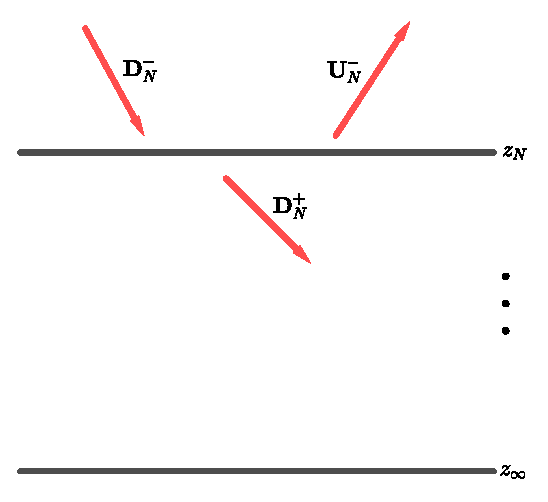
\includegraphics[scale=1]{ondas_em_zn}
\caption{\textit{Ondas ascendentes e descendentes na \'ultima interface.}}
\label{fig.ondas_em_zn}
\end{figure}

Substituindo a equa\c{c}\~ao \ref{eq.inversa_matriz_salto} na equa\c{c}\~ao anterior, temos
\begin{align*}
\begin{pmatrix}
\mathbf{U}_N^-\\
\mathbf{D}_N^-
\end{pmatrix}
&=
\begin{pmatrix}
J_{A,N}^\top&-J_{B,N}^\top\\
-J_{B,N}^\top&J_{A,N}^\top
\end{pmatrix}
\,
\begin{pmatrix}
0\\
\mathbf{D}_N^+
\end{pmatrix}\\\\
&=
\begin{pmatrix}
-J_{B,N}^\top \mathbf{D}_N^+\\
 J_{A,N}^\top \mathbf{D}_N^+
\end{pmatrix},
\end{align*}
ou seja,
\begin{align*}
\mathbf{U}_N^-&=-J_{B,N}^\top J_{A,N}^{-\top}\mathbf{D}_N^-\\
\mathbf{D}_N^+&=J_{A,N}^{-\top}\mathbf{D}_N^-.
\end{align*}
Assim, vemos que para computar uma onda refletida, ou seja, uma onda ascendente a partir de uma interface entre camadas, usamos uma \textit{matriz de reflex\~ao} que fica definida como
\begin{equation}\label{eq.reflexao_N}
\Gamma_N=-J_{B,N}^\top J_{A,N}^{-\top}.
\end{equation} 
Analogamente, vemos que para computar uma onda transmitida, ou seja, uma onda descendente a partir de uma interface entre camadas, usamos uma \textit{matriz de transmiss\~ao} que fica definida como
\begin{equation}\label{eq.transmissao_N}
T_N=J_{A,N}^{-\top}.
\end{equation} 

\subsection{Reflex\~ao e Transmiss\~ao numa Interface Qualquer}
Definimos a espessura de uma camada, a partir da interface superior, como
\begin{equation}
\Delta\,z_m=z_{m+1}-z_m,\qquad m=1,2,...,N-1,
\end{equation}
e temos que uma onda se propagando da interface na profundidade $z_m$ at\'e a interface em $z_{m+1}$ percorre uma profundidade total $\Delta\,z_m$. O valor dessa onda no fim da trajet\'oria, quando $z=z_{m+1}$, \'e aproximadamente igual a $\mathbf{\Psi}^-_{m+1}$, conforme a figura \ref{fig.N_interfaces}. Assim, usando a solu\c{c}\~ao \ref{eq.solucao_psi} podemos escrever
\begin{equation}\label{eq.solucao_delta_zm}
\mathbf{\Psi}^-_{m+1}=e^{-i\,\omega\tilde{\Lambda}_m\Delta\,z_m}\mathbf{\Psi}^+_m.
\end{equation}

\begin{figure}
\centering
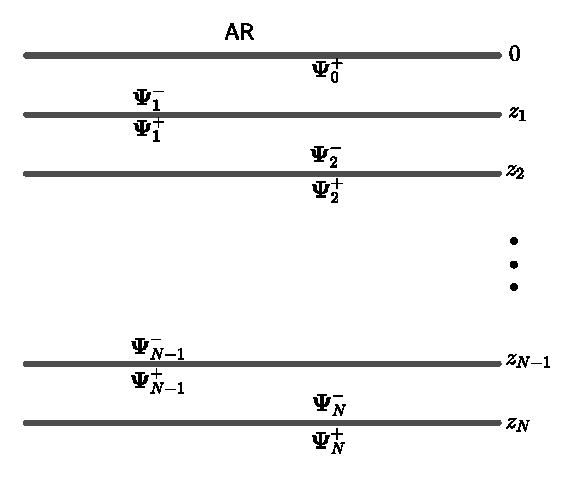
\includegraphics[scale=1]{n_interfaces}
\caption{\textit{Visualizacao de $N$ interfaces em subsuperficie e a notacao das ondas nas proximadades de cada interface.}}
\label{fig.N_interfaces}
\end{figure}

Sabendo que essa onda se propagando na camada abaixo da interface em $z_m$ veio da camada anterior, podemos usar a matriz de salto na equa\c{c}\~ao \ref{eq.psi_matriz_salto} e escrever
\begin{align}\label{eq.salto_m}
\mathbf{\Psi}^+_{m}&=J_m\,\mathbf{\Psi}^-_m.\\
\end{align}
Substituindo a equa\c{c}\~ao \ref{eq.salto_m} na equa\c{c}\~ao \ref{eq.solucao_delta_zm}, temos
\begin{align*}
\mathbf{\Psi}^-_{m+1}&=e^{-i\,\omega\tilde{\Lambda}_m\Delta\,z_m}\mathbf{\Psi}^+_m\\
\mathbf{\Psi}^-_{m+1}&=e^{-i\,\omega\tilde{\Lambda}_m\Delta\,z_m}J_m\,\mathbf{\Psi}^-_m\\
\mathbf{\Psi}^-_m&=J^{-1}_me^{i\,\omega\tilde{\Lambda}_m\Delta\,z_m}\mathbf{\Psi}^-_{m+1}
\end{align*}
Substituindo a equa\c{c}\~ao \ref{eq.definicao_psi} e a equa\c{c}\~ao \ref{eq.inversa_matriz_salto}, temos
\begin{align}\label{eq.refle_trans_1}
\mathbf{U}_m^-&=J^\top_{A,m}e^{i\,\omega\Lambda_m\Delta\,z_m}\mathbf{U}^-_{m+1}-J^\top_{B,m}e^{-i\,\omega\Lambda_m\Delta\,z_m}\mathbf{D}^-_{m+1}\\\nonumber\\\label{eq.refle_trans_2}
\mathbf{D}_m^-&=-J^\top_{B,m}e^{i\,\omega\Lambda_m\Delta\,z_m}\mathbf{U}^-_{m+1}+J^\top_{A,m}e^{-i\,\omega\Lambda_m\Delta\,z_m}\mathbf{D}^-_{m+1}.
\end{align}
Assim como definimos matriz de reflex\~ao para a \'ultima interface em $z_N$, podemos definir a matriz de reflex\~ao para uma interface qualquer, ou seja,
\begin{equation}\label{eq.reflexao_m+1}
\mathbf{U}^-_{m+1}=\Gamma_{m+1}\mathbf{D}^-_{m+1}.
\end{equation}
Substituindo a equa\c{c}\~ao \ref{eq.reflexao_m+1} na equa\c{c}\~ao \ref{eq.refle_trans_1} e na equa\c{c}\~ao \ref{eq.refle_trans_2}, temos
\begin{align}\label{eq.refle_trans_3}
\mathbf{U}_m^-&=(J^\top_{A,m}e^{i\,\omega\Lambda_m\Delta\,z_m}\Gamma_{m+1}-J^\top_{B,m}e^{-i\,\omega\Lambda_m\Delta\,z_m})\mathbf{D}^-_{m+1}\\\nonumber\\\label{eq.refle_trans_4}
\mathbf{D}_m^-&=(-J^\top_{B,m}e^{i\,\omega\Lambda_m\Delta\,z_m}\Gamma_{m+1}+J^\top_{A,m}e^{-i\,\omega\Lambda_m\Delta\,z_m})\mathbf{D}^-_{m+1}\,.
\end{align}
Substituindo a equa\c{c}\~ao \ref{eq.refle_trans_4} na equa\c{c}\~ao \ref{eq.refle_trans_3}, temos
\begin{align*}
\mathbf{U}_m^-&=(J^\top_{A,m}e^{i\,\omega\Lambda_m\Delta\,z_m}\Gamma_{m+1}-J^\top_{B,m}e^{-i\,\omega\Lambda_m\Delta\,z_m})\\
&\,\,\cdot\,\,(-J^\top_{B,m}e^{i\,\omega\Lambda_m\Delta\,z_m}\Gamma_{m+1}+J^\top_{A,m}e^{-i\,\omega\Lambda_m\Delta\,z_m})^{-1}\mathbf{D}_m^-\,,
\end{align*}
de onde podemos concluir que a matriz de reflex\~ao em uma interface em $z_m$ qualquer \'e dada por
\begin{align*}
\Gamma_{m}&=(J^\top_{A,m}e^{i\,\omega\Lambda_m\Delta\,z_m}\Gamma_{m+1}-J^\top_{B,m}e^{-i\,\omega\Lambda_m\Delta\,z_m})\\
&\,\,\cdot\,\,(-J^\top_{B,m}e^{i\,\omega\Lambda_m\Delta\,z_m}\Gamma_{m+1}+J^\top_{A,m}e^{-i\,\omega\Lambda_m\Delta\,z_m})^{-1},
\end{align*}
ou
\begin{align}\nonumber
\Gamma_{m}&=(J^\top_{A,m}e^{i\,\omega\Lambda_m\Delta\,z_m}\Gamma_{m+1}e^{i\,\omega\Lambda_m\Delta\,z_m}-J^\top_{B,m})\\\label{eq.matriz_reflexao_m}
&\,\,\cdot\,\,(-J^\top_{B,m}e^{i\,\omega\Lambda_m\Delta\,z_m}\Gamma_{m+1}e^{i\,\omega\Lambda_m\Delta\,z_m}+J^\top_{A,m})^{-1}.
\end{align}
Quando uma onda atinge uma interface, alem da possibilidade de reflexao ha tambem a possibilidade de trasmissao da onda para a camada inferior. De maneira analoga ao desenvolvido para reflexao de ondas, podemos deduzir a matriz para a transmissao de ondas em uma interface qualquer, que eh dada por
\begin{equation}\label{eq.matriz_transmissao_m}
T_m=T_{m+1}e^{i\,\omega\,\Lambda\Delta\,z_m}(-J^\top_{B,m}e^{i\,\omega\Lambda_m\Delta\,z_m}\Gamma_{m+1}e^{i\,\omega\Lambda_m\Delta\,z_m}+J^\top_{A,m})^{-1}.
\end{equation}
A validade das equacoes \ref{eq.matriz_reflexao_m} e \ref{eq.matriz_transmissao_m} para qualquer interface pode ser demonstrada por inducao sobre $m$, e todas as matrizes de reflexao e transmissao podem ser computadas por recurssao partindo das equacoes \ref{eq.reflexao_N} e \ref{eq.transmissao_N}.





